
% This LaTeX was auto-generated from MATLAB code.
% To make changes, update the MATLAB code and republish this document.

\documentclass[11pt]{article}
\usepackage[utf8]{inputenc}
\usepackage[T1]{fontenc}
\usepackage{amsthm}
\usepackage{enumitem}
\usepackage{amssymb}
\usepackage{amsmath}
\usepackage{amsfonts}
\usepackage[version=4]{mhchem}
\usepackage{stmaryrd}
\usepackage{mathrsfs}
\usepackage{bm}
\usepackage{graphicx}
\usepackage[export]{adjustbox}
%\graphicspath{ {./images/} }
\usepackage{algorithm}
\usepackage{algorithmic}
\usepackage{makecell}  % 表格换行
\usepackage{url}


\usepackage{hyperref}
\hypersetup{
    colorlinks=true,     % 启用颜色链接
    linkcolor=blue,     % 内部链接的颜色
    citecolor=blue,      % 引用文献的颜色
    urlcolor=blue,       % URL链接的颜色
    linktoc=red,      % 不影响目录链接颜色
}

\usepackage[a4paper, top=1in, bottom=1in, left=1in, right=1in]{geometry}

\title{
{\bf \huge Notes on M\"untz-Jackson Theorem}
%{\bf \large For M\"untz systems on [0,1]}
}
\author{Huaijin Wang}
\date{December 24, 2024}


\begin{document}

\newtheorem{definition}{Definition}[section]
\newtheorem{property}{Property}[section]
\newtheorem{theorem}{Theorem}[section]
\newtheorem{aux-thm}{AuxThm}[section]
\newtheorem*{cust-thm}{Theorem}
\newtheorem{lemma}[theorem]{Lemma}
\newtheorem{aux-lem}{AuxLem}[section]
\newtheorem{corollary}[theorem]{Corollary}
\newtheorem{aux-cor}{AuxCor}[section]
\newtheorem{remark}{Remark}[section]
\newtheorem{example}{Example}[]
\newtheorem*{notation}{Notation Declaration}

%\maketitle

\begingroup
\hypersetup{
    linkcolor=black,  % 将目录链接颜色设置为黑色
}
%\tableofcontents
\endgroup

\newpage

\setcounter{section}{1}
\section{M\"untz-Jackson Theorems}
\subsection*{Recall:}

\noindent $\bullet$ \textbf{Density properties of M\"untz polynomials.}
\begin{cust-thm}[\textcolor{blue}{Theorem 1.1} in \cite{lorentz1996}]
\item Let $\Lambda_\infty = \{0=\lambda_0< \lambda_1< \cdots <\lambda_n < \infty \}$ with $\lambda_n\to \infty$. Then the M\"untz space $\mathcal{M}(\Lambda_\infty)$ is dense in each of the spaces $C[0,1]$ or $L_p[0,1]$, $1\leqslant p <\infty$ if and only if
\[
\sum_{k=1}^\infty \frac{1}{\lambda_k} = \infty.
\]
\end{cust-thm}
The density properties can be indeed extended in several ways: unsorted sequences (which may occur different cluster points), complex sequences, and intervals away from the origin.

\vspace{1em}
\noindent $\bullet$ \textbf{$L_p$-Best Approximation by M\"untz Polynomials.}
Let $f\in L_p [0,1]$ if $1\leqslant p < \infty$ (or $C[0,1]$ if $p=\infty$). The error of approximation from $\mathcal{M}(\Lambda_n)$ to $f$ is
\[
E(f,\Lambda_n)_p := \inf_{M\in\mathcal{M}(\Lambda_n)} \|f-M\|_{L_p[0,1]}.
\]

It is well-defined when the $L_\infty$ norm is applied on functions in $C[0,1]$. In fact, when $p=\infty$, for $f\in C[0,1]$ we have 
\[
\|f\|_\infty := \inf \{C: |f(x)|\leqslant C \text{ a.e. on } [0,1]\} = \inf _{\substack{m F_0 = 0 \\F_0\subset [0,1] }} \left\{\sup_{x\in [0,1] \backslash F_0} |f(x)| \right\} = \max_{0\leqslant x\leqslant 1}\{ |f(x)|\},
\]
where $m F_0 = 0$ denotes that the Lebesgue measure of $F_0$ is $0$.

\subsection*{Plan:}
We consider the $L_p$ best approximation (or Jackson Theorems in Sec. 2) in several subsections:
\begin{enumerate}
\item Existence and uniqueness of $L_p$ best approximation.
\item Error of approximation for monomial $x^r$, and dense properties.
\item Error of approximation for $f\in W_p^1[0,1]$, and some corollaries.
\end{enumerate}

\subsection*{Notation Convention:}
\begin{itemize}
\item \textbf{AuxThm} refers to the auxiliary theorem, which is not included in this book, similar to \textbf{AuxCor}, \textbf{AuxLem}, and other related terms.
\item Denote $\Lambda_\infty = \{0=\lambda_0<\lambda_1<\cdots<\lambda_n<\cdots\}$ with $\lim_{n\to\infty} \lambda_n = \infty$.
\item Denote $\Lambda_n=\{0=\lambda_0<\lambda_1<\cdots<\lambda_n\}$ simply by $\Lambda$, where the integer $n\geqslant 1$ is fixed.
\item Denote the linear space $\mathcal{M}(\Lambda_n)=\mathrm{span}\{x^{\lambda_0},\cdots,x^{\lambda_n}\}$, associated to $\Lambda_n$, with respect to the field of real numbers $\mathbb{R}$.
\item $E(f,\Lambda_n)_p = \inf_{M\in \mathcal{M}(\Lambda_n)} \|f-M\|_{p}$, where $\|\cdot\|_p$ stands for the $L_p[0,1]$ norm for $1\leqslant p\leqslant \infty$. 
\end{itemize}


\newpage

\subsection{Existence and uniqueness of $L_p$-best approximation.}
Let $(X,\|\cdot\|)$ be a Banach space with \textbf{real or complex} scalars,  and $X_n \subset{X}$ be its finite dimensional linear subspace. The \textit{best approximation} to $f\in X$ from $X_n$ is defined as
\[
E(f) := \inf_{p\in X_n} \|f-p\|.
\]
\begin{aux-thm}[Theorem 1.1, p.59, \cite{lorentz1993}]
For each $f\in X$, there exists a best approximation to $f$ from $X_n$.
\end{aux-thm}

\begin{aux-thm}
If $X$ is strictly convex, which is characterized by
\[
\left\{\begin{array}{ll}
\forall f_1 \neq f_2, & \left\|f_1\right\|=\left\|f_2\right\|=1, \quad \alpha_1, \alpha_2>0, \quad \alpha_1+\alpha_2=1, \\
\text { imply } & \left\|\alpha_1 f_1+\alpha_2 f_2\right\|<1.
\end{array}\right.
\]
Then the best approximation to $f\in X$ from $X_n$ is \textbf{unique}.
\end{aux-thm}

\begin{aux-lem}
$L_p[a,b]$ is strictly convex for $1<p<\infty$.
\end{aux-lem}

\begin{remark}
Both $L_1[a,b]$ and $L_\infty[a,b]$ are \textbf{not} strictly convex. 
\end{remark}

\begin{remark}
When we consider vectors in $\mathbb{R}^2$, the strictly convex property for $L_p$ is \textbf{visualizable}. Let $\mathbf{x} = [x_1,x_2]$.
\end{remark}

% \includegraphics[width=1\textwidth]{https://wanghuaijin.github.io/assets/discuss24Dec/images/eps1.eps}  
 
\begin{figure}[H]
\centering
    \includegraphics[width=1\textwidth]{eps1.eps}  
    \caption{Unit circles in $\mathbb{R}^2$ with different $L_p$-norm. Download the \href{https://wanghuaijin.github.io/assets/discuss24Dec/images/eps1.eps}{Figure} and  \href{https://wanghuaijin.github.io/assets/discuss24Dec/codes/eps1.eps}{Code}.}
\end{figure}

\begin{aux-thm}
Let $X=C[a,b]$. If $X_n \subset X$ satisfies the \textbf{Haar condition}:
\[
\text{ Let $\{\phi_i(x)\}_{i=1}^n$ be any basis of $X_n$. Then for any set of distinct points $\{\xi_i\}_{i=1}^n \subset [a,b]$, } 
\]
\[
\begin{bmatrix}
\phi_1(\xi_1) & \cdots& \phi_1(\xi_n) \\
\vdots & & \vdots \\
\phi_n(\xi_1) & \cdots & \phi_n(\xi_n)
\end{bmatrix}
\text{  is non-singular.}
\]
Then for any $f\in X$, there is just one $L_1$ (or $L_\infty$) best approximation to $f$ from $X_n$.
\end{aux-thm}

\subsection{Error of approximation for monomial $x^r$.}
\noindent \textbf{Plan of this subsection}:
\begin{itemize}
\item Proves $E(x^r,\Lambda)_2$ (\textcolor{blue}{Eq. (2.1)}) and $\mathcal{M}(\Lambda_\infty)$ is dense in $L_2[0,1]$;
\item Proves $E(x^r,\Lambda)_\infty$ (\textcolor{blue}{Eq. (2.2)}) and $\mathcal{M}(\Lambda_\infty)$ is dense in $C[0,1]$;
\item Proves $E(x^r,\Lambda)_p$ ($2<p<\infty$) (\textcolor{blue}{Theorem 2.2}), and $\mathcal{M}(\Lambda_\infty)$ is dense in $L_p[0,1]$.
\end{itemize}

\subsubsection{Case 1: $p=2$.}
Our goal is to prove \textcolor{blue}{$(2.1)$} in \cite{lorentz1996}, which is stated as following theorem:
\begin{aux-thm}[see also \textcolor{blue}{Theorem 5.4} in \cite{lorentz1993}]  \label{aux-thm-1}
For $r>-1/2$, $\Lambda = \{\lambda_0,\lambda_1,\cdots,\lambda_n\}$ with distinct elements and $\lambda_k > -1/2$, $k=0,1,\cdots,n$, we have
\[
E(x^r, \Lambda)_2 = \frac{1}{\sqrt{2r+1}} \prod_{k={0}}^n \frac{|r-\lambda_k|}{|r+\lambda_k+1|}.
\]
\end{aux-thm}


\noindent \textbf{Preliminaries.}

In a \textbf{real} Hilbert space $(H,(\cdot,\cdot))$ with its norm induced by $\|f\|=\sqrt{(f,f)}$, let $f_1,\cdots,f_n \in H$ be linearly independent elements, and let $X_n := \mathrm{span}\{f_1,\cdots,f_n\}$. 
\begin{aux-thm} \label{aux-thm-2}
For $g\in H$, there is a \textbf{unique} $f \in X_n$ such that 
\[
\|g-f \| = \inf_{p\in X_n} \|g-p \| .
\]
\end{aux-thm}


We call $f$ \textit{the best approximation} of $g$ from $X_n$ in $H$. 

\begin{aux-cor}\label{aux-cor-1}
Let $f$ be the best approximation of $g$, then it is equivalent to orthogonal projection:
\[
(g-f, p) = 0,\quad \forall p\in X_n.
\]
\end{aux-cor}


\begin{aux-lem}\label{aux-lem-1}
The distance of best approximation $d:=\inf_{p\in X_n} \|g-p\|$ is given by
\[
d^2 = \frac{G(g,f_1,\cdots,f_n)}{G(f_1,\cdots,f_n)},
\]
where $G$ is the Gram determinant 
\[
G(f_1,\cdots,f_n) = 
\left |
\begin{array}{ccc}
(f_1,f_1) & \cdots & (f_1,f_n) \\
 \vdots & & \vdots \\
 (f_n, f_1) & \cdots & (f_n,f_n) \\
\end{array}
\right |.
\]
\end{aux-lem}


\begin{remark}
$G(f_1,\cdots,f_n)\neq 0$ if and only if $f_1,\cdots,f_n$ are linearly independent.
\end{remark}

\begin{remark}
AuxThm \ref{aux-thm-2}, AuxCor \ref{aux-cor-1}, and AuxLem \ref{aux-lem-1} provide a \textbf{general framework} to compute error estimation of best approximation in a Hilbert space. 
\end{remark}

\begin{aux-lem}[Cauchy's determinant]
For real numbers $a_i$ and $b_k$ that satisfy $a_i+b_k\neq 0$, $1\leqslant i,k \leqslant n$, we have
\[
\left |
\begin{array}{ccc}
\frac{1}{a_1+b_1} & \cdots & \frac{1}{a_1+b_n} \\
\vdots & & \vdots \\
\frac{1}{a_n+b_1} & \cdots & \frac{1}{a_n+b_n} \\
\end{array}
\right |
=
\frac{\prod_{n \geqslant i>k\geqslant 1} (a_i-a_k)(b_i-b_k)}{\prod_{1\leqslant i,k \leqslant n} (a_i+b_k)}.
\]
\end{aux-lem}

\begin{proof}[Proof of AuxThm \ref{aux-thm-1}]
Note that for $\lambda, \mu > -1/2$, we have 
\[
(x^\lambda, x^\mu)_{L_2(0,1)} = \frac{1}{\lambda+\mu+1}.
\]
Then the theorem follows from
\[
G(x^{\lambda_0},\cdots,x^{\lambda_n}) = \frac{\prod_{n\geqslant i>k\geqslant 0} (\lambda_i-\lambda_k)^2 }{ \prod_{i=0}^n \prod_{k=0}^n (\lambda_i+\lambda_k+1)},
\]
and
\[
G(x^r,x^{\lambda_0},\cdots,x^{\lambda_n}) = G(x^{\lambda_0},\cdots,x^{\lambda_n}) \cdot \frac{\prod_{k=0}^n (r-\lambda_k)^2}{(2r+1) \prod_{k=0}^n (r+\lambda_k+1)^2}.
\]
\end{proof}

\begin{cust-thm}[Part of \textcolor{blue}{Theorem 1.1}]
Let $\Lambda_\infty = \{0=\lambda_0<\lambda_1<\cdots<\lambda_n<\cdots \}$ and $\lim_{n\to\infty} \lambda_n = \infty$. Then $\mathcal{M}(\Lambda_\infty)$ is dense in $L_2[0,1]$ if and only if $\sum_{k=1}^{\infty} \lambda_k^{-1} = \infty$.
\end{cust-thm}

\begin{remark}
Let $a_k>-1$, the convergence or divergence of infinity product can be related to infinity sum:
\begin{itemize}
\item $\prod_k (1+a_k)$ converges if and only if $\sum_k \log (1+a_k)$ converges.
\item $\prod_k (1+a_k)$ diverges to $0$ (or $+\infty$) if and only if $\sum_k \log (1+a_k)$ diverges to $-\infty$ (or $+\infty$). 
\end{itemize}
\end{remark}

\begin{proof}
We note that the space of algebraic polynomials $\mathbb{P}$ is dense in $L_2[0,1]$. It is sufficient to show that
\[
\forall r\in \mathbb{N}=\{0,1,2,\cdots\}, \ \lim_{n\to \infty }E(x^r,\Lambda_n)_2 = 0 \iff \sum_{k=1}^\infty \frac{1}{\lambda_k} = \infty.
\]
"$\Leftarrow$" \textbf{Sufficiency}. Suppose that $\sum_{n=1}^\infty \lambda_n^{-1} = \infty$ and $r \in \mathbb{N} \backslash \Lambda_\infty$.  Note that  $0\in \Lambda_\infty$, thus $r\geqslant 1$. There exists an index $k_0$ s.t. $\lambda_k>r$ whenever $k\geqslant k_0$. Then
\[
\lim_{n\to\infty} E(x^r,\Lambda_n)_2 = \frac{1}{\sqrt{2r+1}} \frac{\prod_{k=0}^\infty |r-\lambda_k|}{\prod_{k=0}^\infty |r+\lambda_k+1|}
= C(r,k_0) \frac{\prod_{k=k_0}^\infty \left (1-\frac{r}{\lambda_k}\right )}{\prod_{k=k_0}^\infty \left (1+ \frac{r+1}{\lambda_k}\right )},
\]
where
\[ C(r,k_0) = \frac{1}{\sqrt{2r+1}} \prod_{k=0}^{k_0-1} \frac{ |r-\lambda_k|}{ |r+\lambda_k+1|}.
\]
Denote 
\[
S_1 = \sum_{k=k_0}^\infty \log\left (1-\frac{r}{\lambda_k} \right),\
S_2 = \sum_{k=k_0}^\infty \log \left( 1+ \frac{r+1}{\lambda_k} \right).
\]
Then $S_1$ diverges to $-\infty$ (or the positive series $-S_1$ diverges to $+\infty$), if and only if the positive series  
\[
\sum_{k=k_0}^\infty \frac{r}{\lambda_k} = +\infty.
\]
Similarly, $S_2$ diverges to $\infty$ if and only if the positive series
\[
\sum_{k=k_0}^\infty \frac{r+1}{\lambda_k} = \infty.
\]
Then $\lim_{n\to\infty} E(x^r,\Lambda_n)_2=0$ is obtained.

\vspace{1em}

\noindent "$\Rightarrow$" \textbf{Necessity}. Otherwise, we suppose that $\sum_{k=1}^\infty \lambda_k^{-1} < \infty$. Then $S_1$ converges to a value ($\neq 0$), and $S_2$ converges to a value ($\neq 0$). Hence $\lim_{n\to\infty} E(x^r,\Lambda_n)_2 \neq 0$ leads to a contradiction.
\end{proof}

\begin{remark}
The value $\lambda_0=0$ can be removed. In fact, let $\Lambda_\infty = \{0<\lambda_1<\cdots<\lambda_n<\cdots\}$ with $\lim_{n\to\infty} \lambda_n=+\infty$, then
\[
\begin{aligned}
\lim_{n\to\infty} E(1, \Lambda_n)_2 = 0 & \iff \prod_{k=1}^\infty \left( 1 - \frac{1}{\lambda_k+1} \right) = 0 \iff \sum_{k=1}^\infty \log \left (1-\frac{1}{\lambda_k+1}\right ) = -\infty \\
& \iff \sum_{k=1}^\infty \frac{1}{\lambda_k+1}  = +\infty
\iff \sum_{k=1}^\infty \frac{1}{\lambda_k}  = +\infty.
\end{aligned}
\]
\end{remark}


\subsubsection{Case 2: $p=\infty$.}
\noindent Our goal is to prove the \textcolor{blue}{$(2.2)$} in \cite{lorentz1996}, which is stated as following theorem:
\begin{aux-thm}[\textcolor{blue}{Theorem 5.5} in \cite{lorentz1993}] \label{aux-thm-3}
For $r>0$, $\Lambda = \{\lambda_1,\lambda_2,\cdots,\lambda_n\}$ with $\lambda_k > 0$, $k=1,\cdots,n$, we have
\begin{equation}
E(x^r, \Lambda)_\infty \leqslant \prod_{k=\textcolor{red}{1}}^n \frac{|r-\lambda_k|}{r+\lambda_k}.
\label{eq-2-5}
\end{equation}
\end{aux-thm}


\begin{proof}
For any \textcolor{red}{$M>0$} (it will be determined later), we put $\bar{r} = M r$ and $\mu_k = M \lambda_k$. For any coefficients $\textcolor{red}{c_k}\in\mathbb{R}$, we set 
\[
b_k = \frac{\bar{r}+1/2}{\mu_k+1/2} c_k, \ k=1,2,\cdots,n,
\]
and obtain
\begin{equation}
x^{\bar{r}+1/2} - \sum_{k=1}^n b_k x^{\mu_k+1/2} = \left (\bar{r}+\frac{1}{2} \right ) \int_0^x \left [ t^{\bar{r}-1/2} - \sum_{k=1}^n c_k t^{\mu_k-1/2} \right ] \mathrm{d} t.
\label{eq-2-3}
\end{equation}
Since $\mu_k-1/2>-1/2$, $k=1,\cdots,n$, by AuxThm \ref{aux-thm-1} we can select $\textcolor{magenta}{c_k}$ to satisfy
\[
\left \|t^{\bar{r}-1/2} - \sum_{k=1}^n c_k t^{\mu_k-1/2} \right \|_{L^2(0,1)}
= \frac{1}{\sqrt{2\bar{r}}} \prod_{k=1}^n \frac{|\bar{r} - \mu_k|}{\bar{r} + \mu_k }.
\]
Then by Cauchy-Schwarz inequality and \eqref{eq-2-3}, we have $\forall x\in [0,1]$ and $M>0$
\[
\left | x^{\bar{r}+1/2} - \sum_{k=1}^n b_k x^{\mu_k+1/2} \right | \leqslant 
\left (\bar{r}+\frac{1}{2} \right ) \sqrt{x} \left \| t^{\bar{r}-1/2} - \sum_{k=1}^n c_k t^{\mu_k-1/2} \right \|_{L^2(0,1)},
\] 
which leads to
\begin{equation}
\left | x^{M r} - \sum_{k=1}^n b_k x^{M \lambda_k} \right | \leqslant 
\frac{Mr + 1/2}{\sqrt{2M r}} \prod_{k=1}^{n} \frac{|r-\lambda_k|}{r+\lambda_k}.
\label{eq-2-4}
\end{equation}
By choosing $\textcolor{magenta}{M = 1/(2r)}$ and taking the transform $u = x^{1/(2r)}$ on \eqref{eq-2-4}, we have $\forall u\in [0,1]$
\[
\left | u^r - \sum_{k=1}^n b_k u^{\lambda_k} \right | \leqslant \prod_{k=1}^n \frac{|r-\lambda_k|}{r+\lambda_k},
\]
which give rise to \eqref{eq-2-5}.
\end{proof}


\begin{cust-thm}[Part of \textcolor{blue}{Theorem 1.1}]
Let $\Lambda_\infty = \{0=\lambda_0<\lambda_1<\cdots<\lambda_n<\cdots\}$ and $\lim_{n\to\infty}\lambda_n=\infty$. Then $\mathcal{M}(\Lambda_\infty)$ is dense in $C[0,1]$ if and only if $\sum_{k=1}^\infty \lambda_k^{-1} = \infty$.
\end{cust-thm}
\begin{remark}
{$\lambda_0=0$ must be included in $\Lambda_\infty$.}
\end{remark}

\begin{proof}
We note that $\mathbb{P}$ is dense in $C[0,1]$. It is sufficient to show that
\[
\forall r\in \mathbb{N}=\{0,1,2,\cdots\}, \ \lim_{n\to \infty }E(x^r,\Lambda_n)_\infty = 0 \iff \sum_{k=1}^\infty \frac{1}{\lambda_k} = \infty.
\]

\noindent "$\Leftarrow$" \textbf{Sufficiency}. Suppose that $\sum_{n=1}^\infty \lambda_n^{-1} = \infty$ and $r \in \mathbb{N} \backslash \Lambda_\infty$. Note that  $0\in \Lambda_\infty$, thus $r\geqslant 1$. There exists an index $k_0$ s.t. $\lambda_k>r$ whenever $k\geqslant k_0$. Then
\[
\lim_{n\to\infty} E(x^r,\Lambda_n)_\infty \leqslant \prod_{k=1}^{\infty} \frac{|r-\lambda_k|}{r+\lambda_k} = C(r, k_0) \frac{\prod_{k=k_0}^\infty \left (1-\frac{r}{\lambda_k}\right )}{\prod_{k=k_0}^\infty \left (1+ \frac{r}{\lambda_k}\right )},
\
\text{where }\
C(r,k_0) = \prod_{k=1}^{k_0-1} \frac{ |r-\lambda_k|}{ |r+\lambda_k|}.
\]
Denote 
\[
S_1 = \sum_{k=k_0}^\infty \log\left (1-\frac{r}{\lambda_k} \right),\
S_2 = \sum_{k=k_0}^\infty \log \left( 1+ \frac{r}{\lambda_k} \right).
\]
Then $S_1$ diverges to $-\infty$ and $S_2$ diverges to $+\infty$, leading to $\lim_{n\to\infty} E(x^r,\Lambda_n)_\infty = 0$.

\vspace{1em}
\noindent "$\Rightarrow$" \textbf{Necessity}. Note that 
\[
E(x^r,\Lambda_n)_\infty \geqslant E(x^r,\Lambda_n)_2.
\]
Then $\forall r\in \mathbb{N}$, $\lim_{n\to\infty} E(x^r,\Lambda_n)_\infty = 0$ gives rise to $\lim_{n\to\infty} E(x^r,\Lambda_n)_2 = 0$, which leads to $\sum_{k=1}^\infty \lambda_k^{-1} = \infty$.
\end{proof}

\subsubsection{Case 3: $2<p<\infty$.}
\noindent Our goal is to prove the \textcolor{blue}{Theorem 2.2} in \cite{lorentz1996}:
\begin{theorem}[\textcolor{blue}{Theorem 2.2} in \cite{lorentz1996}] \label{thm:2:2}
Let $2<p<\infty$ and $\Lambda = \{\lambda_0,\lambda_1, \cdots, \lambda_n \}$ with distinct elements and $\lambda_k>-1/p$. For any $r>-\frac{1}{p}$, we have 
\begin{equation}
E(x^r, \Lambda)_p \leqslant \frac{1 + {1}/{p}}{\left (2r+{2}/{p} \right )^{{1}/{p}}} \prod_{k=0}^n \frac{|r-\lambda_k|}{r+\lambda_k+{2}/{p}}.
\tag{2.4}
\label{eq:2:4}
\end{equation}
\end{theorem}

\begin{lemma}[\textcolor{blue}{Lemma 2.1} in \cite{lorentz1996}] \label{lem:2:1}
Let $1\leqslant q<p<\infty$ and let $-\frac{1}{q} < \ell_0 < \ell_1 < \cdots < \ell_n$. For arbitrary real numbers $a_0,a_1,\cdots,a_n$ and 
\[
b_k := \frac{1+\ell_k+\frac{1}{p}}{1+\frac{1}{p}} a_k,\quad 0\leqslant k\leqslant n,
\]
we have
\begin{equation}
\left \| x^{\frac{1}{q}-\frac{1}{p}} - \sum_{k=0}^n a_k x^{\ell_k+\frac{1}{q}-\frac{1}{p}} \right  \|_p \leqslant \left ( 1+\frac{1}{p} \right ) \left \|1- \sum_{k=0}^n b_k x^{\ell_k} \right \|_q.
\tag{2.3}
\label{eq:2:3}
\end{equation}
\end{lemma}

\begin{proof}
Let us denote $K:=1+\frac{1}{p}$ and for $0<x\leqslant 1$
\[
\begin{aligned}
&Q(x) := \sum_{k=0}^n b_k x^{\ell_k},\quad h(x) := x^{\frac{1}{p}} (1-Q(x)), \\
&g(x) := K x^{\frac{1}{q}-1-\frac{2}{p}} \int_0^x h(t) \mathrm{d} t.
\end{aligned}
\]
One easily verifies that $g$ is the function on the left hand side of \eqref{eq:2:3}. Our goal is to show 
\[
\|g\|_{p} \leqslant K \|1-Q(x) \|_q.
\]
To achieve this goal, we employ Hölder type inequalities.

\vspace{1em}

\noindent \textcolor[gray]{0.6}{Hölder inequality: 
For any $1\leqslant p, q\leqslant$ that satisfy $\frac{1}{p}+\frac{1}{q}=1$. Suppose that $f\in L_p(\Omega)$, $g\in L_q(\Omega)$ and $fg\in L_1(\Omega)$, then
\[
\|fg\|_{L_1(\Omega)} \leqslant \|f\|_{L_p(\Omega)} \|g\|_{L_q(\Omega)}.
\]
}

\noindent Firstly, by Hölder's inequality, we have for $0<x\leqslant 1$,
\[
\begin{aligned}
& |g(x)| \leqslant K x^{\frac{1}{q}-1-\frac{2}{p}} \int_0^x |h(t)|\mathrm{d} t 
\leqslant K x^{\frac{1}{q}-1-\frac{2}{p}} \left( \int_0^x 1 \mathrm{d} t\right )^{1-\frac{1}{q}} \left( \int_0^x |h(t)|^q\right)^{\frac{1}{q}} \\
& = K x^{-\frac{2}{p}} \left ( \int_0^x |h(t)|^q \right )^{\frac{1}{q}}
=: K \left ( \int_0^1 F(x,t) \mathrm{d} t \right )^{\frac{1}{q}}
\end{aligned}
\]
where
\[
F(x,t) := \left \{ 
\begin{aligned}
& x^{-\frac{2q}{p}} |h(t)|^q, &\text{ if}\ 0 \leqslant t < x, \\
& 0, & \text{otherwise} .
\end{aligned}
\right .
\quad
\textcolor[gray]{0.6}{\text{Note that } F(x,t)\in [0,1]\times [0,1].}
\]

\vspace{1em}

\noindent
\textcolor[gray]{0.6}{
Hölder-Minkowski inequality (see \cite[p.4]{bahouri2011}) states: \\
\indent Let $(X_1,\mu_1)$ and $(X_2,\mu_2)$ be two measure spaces and $f$ be a nonnegative measurable function over $X_1\times X_2$. For all $1\leqslant q \leqslant p \leqslant \infty$, we have 
\[
\left \| \| f(x_1,\cdot) \|_{L_q(X_2,\mu_2)} \right \|_{L_p(X_1,\mu_1)} \leqslant 
\left \| \| f(\cdot, x_2) \|_{L_p(X_1,\mu_1)} \right \|_{L_q(X_2,\mu_2)}.
\]
}

\noindent Then by Hölder-Minkowski inequality, we have
\[
\begin{aligned}
\|g \|_p & \leqslant K \left[ \int_0^1 \left(\int_0^1 F(x,t) \mathrm{d} t\right)^{\frac{p}{q}} \mathrm{d} x \right  ]^{\frac{1}{p}}
= K \left \| \| F(x,\cdot)^{\frac{1}{q}} \|_q \right \|_p \\
& \leqslant K \left \| \| F(\cdot, t)^\frac{1}{q} \|_p \right \|_q
= K \left [ \int_0^1 \left( \int_0^1 F(x,t)^{\frac{p}{q}}\mathrm{d} x\right )^{\frac{q}{p}} \mathrm{d} t\right ]^{\frac{1}{q}} \\
& = K \left[ \int_0^1 \left ( \int_{\textcolor{red}{t}}^1 x^{-2} |h(t)|^p \mathrm{d} x \right )^{\frac{q}{p}} \mathrm{d} t\right ]^{\frac{1}{q}} \\
& = K \left[ \int_0^1 |h(t)|^q \left (\frac{1}{t}-1 \right)^{\frac{q}{p}} \mathrm{d} t\right ]^{\frac{1}{q}} 
 \textcolor{red}{\leqslant } K \left[ \int_0^1 |h(t)|^q \left (\frac{1}{t}\right)^{\frac{q}{p}} \mathrm{d} t\right ]^{\frac{1}{q}} \\
 & = K \left [ \int_0^1 |t^{-\frac{1}{p}} h(t)|^{q} \mathrm{d} t \right ]^{\frac{1}{q}}
 = K \left [ \int_0^1 |1-Q(t)|^q \mathrm{d} t \right ]^{\frac{1}{q}}.
\end{aligned}
\]
\textcolor[gray]{0.6}{
where the inequality holds since $0<\frac{q}{p}<1$ and $0<\frac{1}{t}-1 <\infty$ and 
\[
\left( \frac{1}{t}-1\right )^{\frac{q}{p}} \leqslant \left( \frac{1}{t} \right )^{\frac{q}{p}}.
\]
}
\end{proof}

\begin{remark}
Note that $q<p$, then Lemma \ref{lem:2:1} is some kind of Inverse Inequality: Higher regularity norm bounded by lower regularity norm.
\end{remark}

\vspace{2em}

\begin{proof}[Proof of Theorem \ref{thm:2:2}]
To prove \eqref{eq:2:4}, our goal is to employ Lemma \ref{lem:2:1} and construct the formula
\[
E(x^r,\Lambda)_p \leqslant \left \| x^{\frac{1}{2}-\frac{1}{p}} - \sum_{k=0}^n a_k x^{\ell_k + \frac{1}{2}-\frac{1}{p}} \right \|_p, \ \text{ for some}\ \textcolor{red}{\ell_k}>-\frac{1}{2} \text{ and } \textcolor{red}{a_k}.
\]
To achieve this, for any $a_k$, $0\leqslant k\leqslant n$, \textcolor[gray]{0.6}{which will be determined later}, we have
\[
E(x^r,\Lambda)_p \leqslant \|x^r - \sum_{k=0}^n a_k x^{\lambda_k} \|_p
= \left [ \int_0^1 \left( x^r - \sum_{k=0}^n a_k x^{\lambda_k} \right )^p \mathrm{d} x \right ]^{\frac{1}{p}}.
\]
By a variable transform $x = y^{\rho}$, $\textcolor{red}{\rho}>0$, \textcolor[gray]{0.6}{which is invariant under the interval $[0,1]$ and $\rho$ will be determined later}, we have
\[
\begin{aligned}
E(x^r,\Lambda)_p & \leqslant \left [ \int_0^1 \left( y^{\rho r} - \sum_{k=0}^n a_k y^{\rho \lambda_k} \right )^p \rho y^{\rho-1} \mathrm{d} y \right ]^{\frac{1}{p}}. \\
& = \rho^{\frac{1}{p}} \left \| y^{\rho r+\frac{\rho}{p} - \frac{1}{p}} - \sum_{k=0}^n a_k y^{\rho \lambda_k + \frac{\rho}{p}-\frac{1}{p}} \right \|_p.
\end{aligned}
\] 
Let $\rho r + \frac{\rho}{p}=\frac{1}{2}$, we obtain $\textcolor{magenta}{\rho} = \frac{p}{2 (pr+1)}$. Let $\textcolor{magenta}{\ell_k} = \frac{p(\lambda_k-r)}{2(pr+1)} > -\frac{1}{2}$, \textcolor[gray]{0.6}{it is easy to examine that $l_k+1/2>0$,} by Lemma \ref{lem:2:1}, we have
\begin{equation}
\begin{aligned}
E(x^r,\Lambda)_p & \leqslant \left( \frac{p}{2(pr+1)}\right )^{\frac{1}{p}}
\left \| y^{\frac{1}{2}-\frac{1}{p}} - \sum_{k=0}^n a_k y^{\ell_k+\frac{1}{2}-\frac{1}{p}} \right \|_p \\
& \leqslant \left( \frac{p}{2(pr+1)}\right )^{\frac{1}{p}} \left( 1+\frac{1}{p} \right ) \left \|  1-\sum_{k=0}^n b_k y^{\ell_k} \right \|_2.
\end{aligned}
\label{eq-2-6}
\end{equation}
Since $a_k$ is arbitrary, hence $\textcolor{red}{b_k}$ is also arbitrary. Take the infimum on the right hand side of \eqref{eq-2-6} over $\textcolor{magenta}{b_k}$, and by Theorem \ref{aux-thm-1}, we have 
\[
E(x^r,\Lambda)_p \leqslant \left( \frac{p}{2(pr+1)}\right )^{\frac{1}{p}} \left( 1+\frac{1}{p} \right ) \prod_{k=0}^n \frac{|\ell_k|}{\ell_k+1} = \frac{1+1/p}{(2r+2/p)^{1/p}} \prod_{k=0}^n \frac{|r-\lambda_k|}{r+\lambda_k+2/p}.
\]
\end{proof}


\begin{cust-thm}[Part of \textcolor{blue}{Theorem 1.1}]
Let $\Lambda_\infty = \{0=\lambda_0<\lambda_1<\cdots<\lambda_n<\cdots \}$ and $\lim_{n\to\infty} \lambda_n = \infty$. Then $\mathcal{M}(\Lambda_\infty)$ is dense in $L_p[0,1]$, $2< p < \infty$, if and only if $\sum_{k=1}^{\infty} \lambda_k^{-1} = \infty$.
\end{cust-thm}
\begin{proof}
We note that $\mathbb{P}$ is dense in $L_p[0,1]$. It is sufficient to show that
\[
\forall r\in \mathbb{N}=\{0,1,2,\cdots\}, \ \lim_{n\to \infty } E(x^r,\Lambda_n)_p = 0 \iff \sum_{k=1}^\infty \frac{1}{\lambda_k} = \infty.
\]

\noindent
"$\Leftarrow$" \textbf{Sufficiency}. Suppose that $\sum_{n=1}^\infty \lambda_n^{-1} = \infty$ and $r \in \mathbb{N} \backslash \Lambda_\infty$.  Note that  $0\in \Lambda_\infty$, thus $r\geqslant 1$. There exists an index $k_0$ s.t. $\lambda_k>r$ whenever $k\geqslant k_0$. Then
\[
\lim_{n\to\infty} E(x^r,\Lambda_n)_p \leqslant \frac{1+1/p}{({2r+2/p})^{1/p}} \frac{\prod_{k=0}^\infty |r-\lambda_k|}{\prod_{k=0}^\infty |r+\lambda_k+2/p|}
= C(r,k_0) \frac{\prod_{k=k_0}^\infty \left (1-\frac{r}{\lambda_k}\right )}{\prod_{k=k_0}^\infty \left (1+ \frac{r+2/p}{\lambda_k}\right )},
\]
where
\[ C(r,k_0) = \frac{1+1/p}{({2r+2/p})^{1/p}} \prod_{k=0}^{k_0-1} \frac{ |r-\lambda_k|}{ |r+\lambda_k+2/p|}.
\]
Denote 
\[
S_1 = \sum_{k=k_0}^\infty \log\left (1-\frac{r}{\lambda_k} \right),\
S_2 = \sum_{k=k_0}^\infty \log \left( 1+ \frac{r+2/p}{\lambda_k} \right).
\]
Then $S_1$ diverges to $-\infty$ and $S_2$ diverges to $+\infty$, leading to obtain $\lim_{n\to\infty} E(x^r,\Lambda_n)_p=0$.

\vspace{1em}

\noindent "$\Rightarrow$" \textbf{Necessity}. Note that 
\[
E(x^r,\Lambda_n)_p \geqslant E(x^r,\Lambda_n)_2.
\]
Then $\forall r\in \mathbb{N}$, $\lim_{n\to\infty} E(x^r,\Lambda_n)_p = 0$ gives rise to $\lim_{n\to\infty} E(x^r,\Lambda_n)_2 = 0$, which leads to $\sum_{k=1}^\infty \lambda_k^{-1} = \infty$.
\end{proof}


\begin{remark}
The value $\lambda_0=0$ can be removed. In fact, let $\Lambda_\infty = \{0<\lambda_1<\cdots<\lambda_n<\cdots\}$ with $\lim_{n\to\infty} \lambda_n=+\infty$,
\[
\begin{aligned}
 &\prod_{k=1}^\infty \left( 1 - \frac{2/p}{\lambda_k+2/p} \right) = 0 \iff \sum_{k=1}^\infty \log \left (1-\frac{2/p}{\lambda_k+2/p}\right ) = -\infty \\
& \iff \sum_{k=1}^\infty \frac{2/p}{\lambda_k+2/p}  = +\infty
\iff \sum_{k=1}^\infty \frac{1}{\lambda_k}  = +\infty.
\end{aligned}
\]
Then if $\sum_{k=1}^\infty \lambda_k^{-1} = \infty$, we have $\lim_{n\to\infty} E(1,\Lambda_n)_p = 0$. Conversely, if $\lim_{n\to\infty} E(1,\Lambda_n)_p = 0$, which leads to $\lim_{n\to\infty} E(1,\Lambda_n)_2 = 0$, we have $\sum_{k=1}^\infty \lambda_k^{-1} = \infty$.
\end{remark}

\subsubsection{Conclusion and remarks.}
Let $2\leqslant p \leqslant \infty$ and $\Lambda = \{\lambda_k\}_{k=0}^n$ with $\lambda_k > -1/p$. Then for any $r>-1/p$, we have
\[
E(x^r,\Lambda)_p \leqslant \frac{1+{1}/{p}}{(2r+2/p)^{1/p}} \prod_{k=0}^{n} \frac{|r-\lambda_k|}{r+\lambda_k+2/p}.
\]

\noindent \textbf{A Variant of Dense Property.}

\noindent (see also Section 5 of Chapter 11 in \cite{lorentz1993})

\noindent Let $C[0,+\infty]$ be the space of continuous functions on $[0,+\infty]$, which have a finite limit for $t\to \infty$. Exponential sums
\[
\sum_{k=0}^n a_k e^{-\lambda_k t}
\]
approximate arbitrarily closely each function $f\in C[0,+\infty]$ if and only if $\lambda_0=0$ and $\sum_{k=1}^\infty \lambda_k^{-1} = \infty$.
\newpage

\begin{thebibliography}{99}
\bibitem[Lorentz (1996)]{lorentz1996} \href{https://wanghuaijin.github.io/assets/discuss24Dec/Lorentz1996.pdf}{Lorentz G G, von Golitschek M, Makovoz Y. Constructive approximation: advanced problems[M]. Berlin: Springer, 1996.}
\bibitem[Erd\'elyi (2001)]{erdelyi2001} \href{https://wanghuaijin.github.io/assets/discuss24Dec/Erdelyi2001.pdf}{Erdélyi T, Johnson W B. The “Full Müntz Theorem” in $L_p [0, 1]$ for $0< p<\infty$ [J]. Journal D’Analyse Mathématique, 2001, 84(1): 145-172.}
\bibitem[Almira (2007)]{almira2007} \href{https://wanghuaijin.github.io/assets/discuss24Dec/Almira2007.pdf}{Almira J M. Muntz type theorems I[J]. arXiv preprint arXiv:0710.3570, 2007.}
\bibitem[Agler (2022)]{agler2022} \href{https://wanghuaijin.github.io/assets/discuss24Dec/Agler2022.pdf}{Agler J, McCarthy J. Asymptotic M\"untz-Sz\'asz Theorems[J]. arXiv preprint arXiv:2206.12487, 2022.}
\bibitem[Wang Renhong (1999)]{wang1999} \href{https://wanghuaijin.github.io/assets/discuss24Dec/Wang1999.pdf}{Wang Renhong. Numerical Approximation (in Chinese)[M]. Higher Education Press, 1999.}
\bibitem[Lorentz (1993)]{lorentz1993} \href{https://wanghuaijin.github.io/assets/discuss24Dec/Lorentz1993.pdf}{DeVore R A, Lorentz G G. Constructive Approximation[M]. Springer-Verlag, 1993.}
\bibitem[Bahouri (2011)]{bahouri2011} \href{https://wanghuaijin.github.io/assets/discuss24Dec/Bahouri2011.pdf}{Bahouri H. Fourier Analysis and Nonlinear Partial Differential Equations[M]. Grundlehren der Mathematischen Wissenschaften, 2011, 343.}
\bibitem[Adams (2003)]{adams2003} \href{https://wanghuaijin.github.io/assets/discuss24Dec/Adams2003.pdf}{Adams R A, Fournier J J F. Sobolev spaces[M]. Elsevier, 2003.}
\bibitem[Borwein (1995)]{borwein1995} \href{https://wanghuaijin.github.io/assets/discuss24Dec/Borwein1995.pdf}{Borwein P, Erdelyi T. Polynomials and Polynomial Inequalities[M]. Springer Science \& Business Media, 1995.}
\bibitem[Powell (1981)]{powell1981} \href{https://wanghuaijin.github.io/assets/discuss24Dec/Powell1981.pdf}{Powell M J D. Approximation theory and methods[M]. Cambridge university press, 1981.}
\bibitem[Brezis (2011)]{brezis2011} \href{https://wanghuaijin.github.io/assets/discuss24Dec/Brezis2011.pdf}{Brezis H. Functional analysis, Sobolev spaces and partial differential equations[M]. New York: Springer, 2011.}
\end{thebibliography}

\end{document}

